\section{Intraprocedural Profiling}

{\em Path profiling} is a powerful {\em intraprocedural} methodology for identifying performance bottlenecks in a program, and has received considerable attention in the last 15 years for its practical relevance. The well-known Ball and Larus numbering algorithm~\cite{Ball96} can efficiently encode {\em acyclic} paths that are taken across the control-flow graph of a function. Previous attempts to extend it to {\em cyclic} paths, as spanning multiple loop iterations, to capture more optimization opportunities, are based on rather complex algorithms that incur severe performance overheads even for short cyclic paths. In this thesis we present a new, data-structure based approach to {\em multi-iteration} path profiling built on top of the original Ball-Larus numbering technique. Starting from the observation that a cyclic path can be described as a concatenation of Ball-Larus acyclic paths, we show how to accurately profile all executed paths obtained as a concatenation of up to $k$ Ball-Larus paths, where $k$ is a user-defined parameter.

%{\em Path profiling} is a powerful {\em intraprocedural} methodology for identifying performance bottlenecks in a program, and has received considerable attention in the last 15 years for its practical relevance. The well-known Ball and Larus algorithm~\cite{Ball96} for {\em intraprocedural} path profiling can efficiently encode {\em acyclic} paths that are taken across the control-flow graph of a function. Previous attempts to extend it to encode {\em cyclic} paths, and thus to span multiple loop iterations in order to capture more optimization opportunities, are based on rather complex algorithms that incur severe performance overheads even for short cyclic paths. In this thesis we present a new, data-structure based approach to {\em multi-iteration} path profiling built on top of the original Ball-Larus numbering technique. Starting from the observation that any cyclic path can be described as a concatenation of Ball-Larus acyclic paths, we show how to accurately profile all executed paths obtained as a concatenation of up to $k$ Ball-Larus paths, where $k$ is a user-defined parameter.

%We provide examples showing that this method can reveal optimization opportunities that acyclic-path profiling would miss, and we present an extensive experimental investigation on a large variety of Java benchmarks in the Jikes RVM. Experiments show that our approach can be even faster than a hash table-based implementation of the Ball-Larus algorithm due to fewer operations on smaller tables, producing compact representations of cyclic paths even for large values of $k$.

\subsection{Motivation and Contributions}

Path profiling associates performance metrics, usually frequency counters, to paths taken in the control flow graph of a routine. Identifying the hottest paths can direct optimizations to portions of the code where most resources are consumed, often yielding significant speedups. For instance, trace scheduling can improve performance by increasing instruction-level parallelism along frequently executed paths~\cite{Fisher81,Young98}. Although basic block and edge profiles are inexpensive and widely available, they do not always correctly predict frequencies of overlapping paths. 

The seminal paper by Ball and Larus~\cite{Ball96} introduced a simple and elegant path profiling technique. The main idea was to implicitly number all possible acyclic paths in the control flow graph so that each path is associated with a unique compact path identifier (ID). The authors showed that path IDs can be efficiently generated at runtime and can be used to update a table\footnote{Large routines can have too many potential paths to use an array of counters. In this case, a slower (but more space-efficient) hash table is used to record only paths that actually execute~\cite{Ball96}.} of frequency counters. Although in general the number of acyclic paths may grow exponentially with the graph size, in typical control flow graphs this number is usually small enough to fit in current machine word-sizes, making this approach very effective in practice.

While the original Ball-Larus approach was restricted to acyclic paths obtained by cutting paths at loop back edges, profiling paths that span consecutive loop iterations is a desirable, yet difficult, task that can yield better optimization opportunities. Consider, for instance, the problem of eliminating redundant executions of instructions, such as loads and stores~\cite{Bodik99}, conditional jumps~\cite{Bodik97}, expressions~\cite{Bodik98,Bodik04}, and array bounds checks~\cite{Bodik00}. A typical situation is that the same instruction is redundantly executed at each loop iteration, which is particularly common for arithmetic expressions and load operations~\cite{Bodik04,Bodik99}. To identify such redundancies, paths that extend across loop back edges need to be profiled. Another application is trace scheduling~\cite{Young98}: if a frequently executed cyclic path is found, compilers may unroll the loop and perform trace scheduling on the unrolled portion of code. Tallam {\em et al.}~\cite{Tallam04} provide a comprehensive discussion of the benefits of multi-iteration path profiling.

Different authors have proposed techniques to profile cyclic paths by modifying the original Ball-Larus path numbering scheme in order to identify paths that extend across multiple loop iterations~\cite{Tallam04,Roy09,Li12}. Unfortunately, all known solutions require rather complex algorithms that incur severe performance overheads even for short cyclic paths, leaving the interesting open question of finding simpler and more efficient alternative methods.

\paragraph*{Contributions.} In this thesis, we present a novel, data structure-based approach to multi-iteration path profiling. Our method stems from the observation that any cyclic execution path in the control flow graph of a routine can be described as a concatenation of Ball-Larus acyclic paths (BL paths). In particular, we show how to accurately profile {\em all executed paths} obtained as a concatenation of up to $k$ BL paths, where $k$ is a user-defined parameter. We reduce multi-iteration path profiling to the problem of counting $n$-grams, i.e., contiguous sequences of $n$ items from a given sequence. To compactly represent collected profiles, we organize them in a forest of prefix trees (or tries)~\cite{Fredkin60} of depth up to $k$, where each node is labeled with a BL path, and paths in a tree represent concatenations of BL paths that were actually executed by the program, along with their frequencies. We also present an efficient construction algorithm based on a variant of the \ksf\ data structure presented in~\cite{Ausiello12}. 

\subsection{Approach}

Differently from previous techniques~\cite{Tallam04,Roy09,Li12}, which rely on modifying the Ball-Larus path numbering to cope with cycles, our method does not	require any modification of the original numbering technique described in~\cite{Ball96}.

\ifdefined\noauthorea
\begin{wrapfigure}[19]{l}{0.5\textwidth}
\vspace{-3mm}
\centering
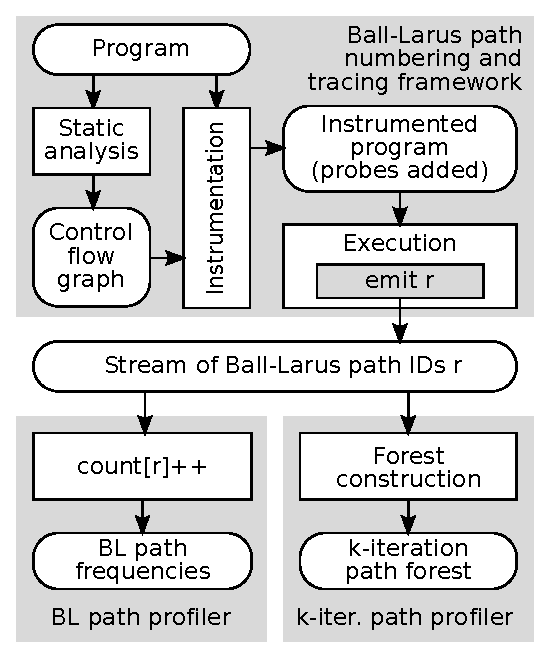
\includegraphics[width=0.433\textwidth]{figures/kblpp-approach/kblpp-approach.eps}
\captionsetup{width=.47\textwidth}
\caption{\protect\label{fig:kblpp-approach} Overview of our approach: Ball-Larus profiling versus k-iteration path profiling, cast in a common framework.
%Overview of our approach: classical Ball-Larus profiling versus k-iteration path profiling, cast in a common framework.
}
%\vspace{2mm}
\end{wrapfigure}
\noindent
\fi

\vspace{-2mm}
\noindent The main idea behind our approach is to fully decouple the task of tracing Ball-Larus acyclic paths at run time from the task of concatenating and storing them in a data structure to keep track of multiple iterations. \myfigure\ref{fig:kblpp-approach} illustrates from a high-level point of view our two-stage process:
\begin{enumerate}[parsep=0pt,itemsep=3pt,topsep=5pt]
\item instrumentation and execution of the program to be profiled;
\item profiling of paths.
\end{enumerate}
We let the Ball-Larus profiling algorithm issue a stream of BL path IDs, where each ID is generated when a back edge in the control flow graph is traversed or the current procedure is abandoned. As a consequence of this modular approach, our method can be implemented on top of existing Ball-Larus path profilers, making it simpler to code and maintain.

%\vspace{1em}

\noindent The first phase is almost identical to the original approach described in~\cite{Ball96}. The target program is statically analyzed and a control flow graph (CFG) is constructed for each routine of interest. The CFG is used to instrument the original program by inserting probes, which allow paths to be traced at run time. When the program is executed, taken acyclic paths are identified using the inserted probes. The main difference with the Ball-Larus approach is that, instead of directly updating a frequency counters table here, we emit a stream of path IDs, which is passed along to the next stage of the process. This allows us to decouple the task of tracing taken paths from the task of profiling them. 

The profiling phase can be either the original hash table-based method of~\cite{Ball96} used to maintain BL path frequencies
%for larger programs
(bottom-left of \myfigure\ref{fig:kblpp-approach}), or other approaches such as the one we propose, i.e., profiling concatenations of BL paths in a forest-based data structure (bottom-right of \myfigure\ref{fig:kblpp-approach}). Different profiling methods can be therefore cast into a common framework, increasing flexibility and helping us make more accurate comparisons.

We start with a brief overview of the Ball-Larus path tracing technique, which we use as the first stage of our profiler.

\subsection{Ball-Larus Path Tracing Algorithm}

The Ball-Larus path profiling (BLPP) technique~\cite{Ball96} identifies each acyclic path that is executed in a routine. Paths start on the method entry and terminate on the method exit. Since loops make the CFG cyclic, loop back edges are substituted by a pair of dummy edges: the first one from the method entry to the target of the loop back edge, and the second one from the source of the loop back edge to the method exit. After this (reversible) transformation, the CFG of a method becomes a DAG (directed acyclic graph) and acyclic paths can be enumerated.

\ifdefined\noauthorea
\begin{figure}[h!]
\IncMargin{2em}
\begin{algorithm}[H]
\DontPrintSemicolon
\LinesNumbered
\SetAlgoNoLine
\SetNlSkip{1em} 
\Indm\Indmm
\hrulefill\\
$\mathbf{procedure} \> \> \texttt{bl\_path\_numbering}$():\;
\vspace{1mm}
\everypar={\nl}
\Indp\Indpp
\ForEach{$\textsf{\rm basic block}$ $v$ $\textsf{\rm in reverse topological order}$}{
    \eIf{$v$ $\textsf{\rm is the exit block}$}{
	numPaths($v$) $\gets 1$\;
    }{
	numPaths($v$) $\gets 0$\;
	\ForEach{$\textsf{\rm outgoing edge}$ $e = (v, w)$}{
	    val($e$) = numPaths($v$) \;
	    numPaths($v$) += numPaths($w$) \;
	}
    }
}
\vspace{-2mm}
\Indm\Indmm
\nonl\hrulefill\vspace{1mm}\\
\DecMargin{5em}
\caption{\label{alg:kblpp-bl-numbering} The Ball-Larus path numbering algorithm.}
\IncMargin{3em}
\end{algorithm}
\end{figure}

\else
\begin{figure}[h!]
\caption{\label{alg:kblpp-bl-numbering} The Ball-Larus path numbering algorithm.}
\begin{small}
\begin{minipage}{0.9\textwidth}
\hrulefill\\
\textbf{procedure} {\tt bl\_path\_numbering}(): \\
\vspace{-2mm}

1. ~~ \textbf{foreach} basic block $v$ in reverse topological order \textbf{do}\\
2. ~~ ~~~~ \textbf{if} $v$ is the exit block \textbf{then}\\
3. ~~ ~~~~ ~~~~ numPaths($v$) $\gets 1$\\
4. ~~ ~~~~ \textbf{else}\\
5. ~~ ~~~~ ~~~~ numPaths($v$) $\gets 0$\\
6. ~~ ~~~~ ~~~~ \textbf{foreach} outgoing edge $e = (v, w)$ \textbf{do}\\
7. ~~ ~~~~ ~~~~ ~~~~ val($e$) = numPaths($v$)\\
8. ~~ ~~~~ ~~~~ ~~~~ numPaths($v$) += numPaths($w$)\\
9. ~~ ~~~~ ~~~~ \textbf{end}\\
10. ~~ ~~~~ \textbf{end}\\
11. ~~ \textbf{end}\\
\vspace{-1mm}
\hrulefill
\vspace{-2mm}
\end{minipage}
\end{small}
\end{figure}

\fi

\ifauthorea{\newline}{}
\noindent The Ball-Larus path numbering algorithm
\ifauthorea{, shown in \myalgorithm\ref{alg:kblpp-bl-numbering},}{(\myalgorithm\ref{alg:kblpp-bl-numbering})}
assigns a value $val(e)$ to each edge $e$ of the CFG such that, given N acyclic paths, the sum of the edge values along any entry-to-exit path is a unique numeric ID in [0, N-1]. A CFG example and the corresponding path IDs are shown in \myfigure\ref{fig:kblpp-example}: notice that there are eight distinct acyclic paths, numbered from 0 to 7, starting either at the method's entry $A$, or at loop header $B$ (target of back edge $(E,B)$).

BLPP places instrumentation on edges to compute a unique path number for each possible path. In particular, it uses a variable {\tt r}, called {\em probe} or {\em path register}, to compute the path number. Variable {\tt r} is first initialized to zero upon method entry and then is updated as edges are traversed. When an edge that reaches the method exit is executed, or a back edge is traversed, variable {\tt r} represents the unique ID of the taken path. As observed, instead of using the path ID {\tt r} to increase the path frequency counter ({\tt count[r]++}), we defer the profiling stage by emitting the path ID to an output stream ({\tt emit r}). To support profiling over multiple invocations of the same routine, we annotate the stream with the special marker $*$ to denote a routine entry event. Instrumentation code for our CFG example is shown on the left of \myfigure\ref{fig:kblpp-example}.

\ifdefined\noauthorea
\begin{figure}[hb]
\begin{center}
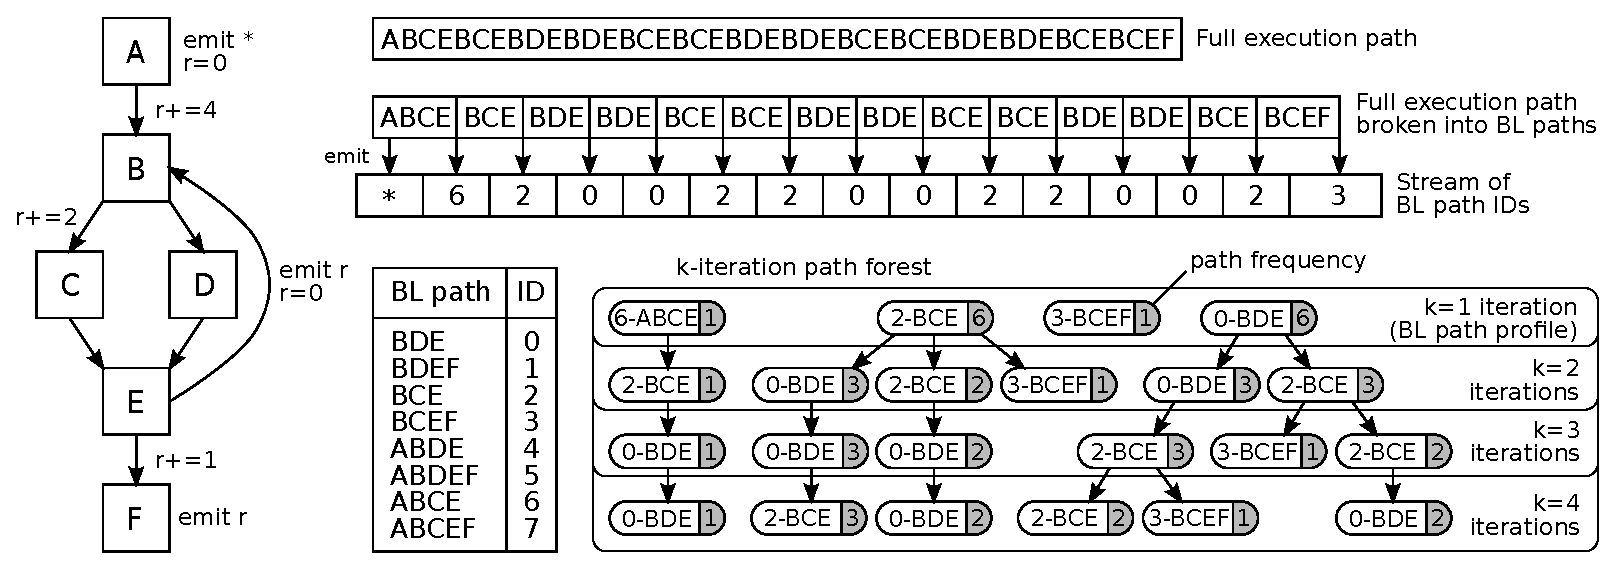
\includegraphics[width=\textwidth]{figures/kblpp-example/kblpp-example.eps}
\caption{\protect\label{fig:kblpp-example} Control flow graph (CFG) with Ball-Larus instrumentation modified to emit acyclic path IDs to an output stream and running example of our approach that shows a 4-iteration path forest (4-IPF) for a possible small execution trace. Loop back edges in the CFG have been restored after the path numbering phase.
}
\end{center}
\end{figure}
\fi

%~\cite{}

\subsection{Algorithms}

\subsection{Discussion}

\subsection{Comparison with Related Work}